\documentclass[12pt,a4paper]{article}
\usepackage[margin=1in]{geometry}
\usepackage{graphicx}
\usepackage{tikz}
\usetikzlibrary{shapes.geometric, arrows, positioning, fit, backgrounds}
\usepackage{enumitem}
\usepackage{booktabs}
\usepackage{hyperref}
\usepackage{xcolor}
\usepackage{tcolorbox}
\usepackage{float}

% Define colors
\definecolor{ruetblue}{RGB}{0,51,102}
\definecolor{lightgray}{RGB}{245,245,245}

\begin{document}

% ============================================
% COVER PAGE
% ============================================
\begin{titlepage}
    \centering
    \vspace*{1cm}
    
    {\Large\textbf{Rajshahi University of Engineering \& Technology}}\\[0.5cm]
    {\large Department of Computer Science \& Engineering}\\[2cm]
    
    \rule{\linewidth}{0.5mm}\\[0.4cm]
    {\Huge\bfseries Payment Processing Module Design}\\[0.3cm]
    {\Large\textbf{Project: Bongoportus}}\\[0.2cm]
    {\large A Multi-Vendor P2P E-Commerce Platform}\\
    \rule{\linewidth}{0.5mm}\\[1.5cm]
    
    {\Large\textbf{CSE 3206 - Software Engineering Sessional}}\\[0.3cm]
    {\large Project Review (CO2, PO3, K5, P1, P6)}\\[2cm]
    
    \begin{minipage}{0.45\textwidth}
        \begin{flushleft}
            \textbf{Submitted By:}\\[0.3cm]
            Name: Umor Faruk\\[0.3cm]
            Roll No: 2103130\\[0.3cm]
            Series: 20\\[0.3cm]
            Department: CSE, RUET
        \end{flushleft}
    \end{minipage}
    \hfill
    \begin{minipage}{0.45\textwidth}
        \begin{flushright}
            \textbf{Submitted To:}\\[0.3cm]
            Farjana Parvin\\[0.2cm]
            Assistant Professor\\[0.2cm]
            Department of CSE\\[0.2cm]
            RUET
        \end{flushright}
    \end{minipage}
    
    \vfill
    {\large Submission Date: January 2026}
\end{titlepage}

% ============================================
% TABLE OF CONTENTS
% ============================================
\tableofcontents
\newpage

% ============================================
% 1. INTRODUCTION (Problem Description)
% ============================================
\section{Introduction}

Bangladesh's e-commerce sector has experienced exponential growth, with platforms handling millions of transactions daily. The \textbf{Bongoportus} platform is a national multi-vendor e-commerce system that supports multiple payment methods including:

\begin{itemize}
    \item \textbf{Mobile Banking:} bKash, Nagad, Upay
    \item \textbf{Card Payments:} Visa, Mastercard
    \item \textbf{Cash on Delivery (COD)}
\end{itemize}

During flash sales and special offers like \textit{New Year Sales} or \textit{Eid promotions}, the system must handle thousands of concurrent payment requests while ensuring:
\begin{itemize}
    \item No duplicate charges to customers
    \item Fast response times under 3 seconds
    \item Complete audit trails for financial compliance
    \item High availability (99.9\% uptime)
\end{itemize}

% IMAGE 1: Homepage
\begin{figure}[H]
    \centering
    \includegraphics[width=0.9\textwidth]{results/homepage.png}
    \caption{Bongoportus E-Commerce Platform Home Page}
    \label{fig:homepage}
\end{figure}

% ============================================
% 2. PROCESS MODEL (2.0 Marks)
% ============================================
\section{Software Process Model Selection}

\subsection{Chosen Model: Agile (Scrum)}

For the payment processing module, we have selected the \textbf{Agile methodology with Scrum framework}. This choice is justified by the following factors:

\begin{tcolorbox}[colback=lightgray,colframe=ruetblue,title=\textbf{Justification for Agile}]
\begin{enumerate}[leftmargin=*]
    \item \textbf{Stakeholder Involvement:}
    \begin{itemize}
        \item Payment systems require continuous feedback from multiple stakeholders: customers, merchants, bank partners, and regulatory bodies
        \item Sprint reviews (every 2 weeks) allow stakeholders to validate payment flows
        \item Product Owner maintains prioritized backlog based on stakeholder needs
    \end{itemize}
    
    \item \textbf{Changing Requirements:}
    \begin{itemize}
        \item Payment gateway APIs frequently update (bKash API v2.0, Nagad integration changes)
        \item New payment methods may be added (e.g., Rocket, bank transfers)
        \item Regulatory changes require quick adaptation (Bangladesh Bank guidelines)
        \item Agile embraces change even late in development
    \end{itemize}
    
    \item \textbf{Testing and Reliability:}
    \begin{itemize}
        \item Test-Driven Development (TDD) ensures payment logic is thoroughly tested
        \item Continuous Integration catches bugs early
        \item Each sprint delivers a potentially shippable increment
        \item Payment failures can be quickly identified and fixed
    \end{itemize}
    
    \item \textbf{Risk Management:}
    \begin{itemize}
        \item Iterative development reduces risk of complete failure
        \item Early prototypes validate integration with external payment gateways
        \item Security testing happens continuously, not just at the end
    \end{itemize}
\end{enumerate}
\end{tcolorbox}

\subsection{Why Not Other Models?}

\begin{table}[H]
\centering
\begin{tabular}{|l|p{8cm}|}
\hline
\textbf{Model} & \textbf{Reason for Rejection} \\
\hline
Waterfall & Too rigid; cannot accommodate payment API changes \\
\hline
Spiral & Overkill for module-level development; better for large systems \\
\hline
Incremental & Lacks the stakeholder feedback loops crucial for payment validation \\
\hline
\end{tabular}
\caption{Comparison with other process models}
\end{table}

% ============================================
% 3. REQUIREMENTS (2.0 Marks)
% ============================================
\section{System Requirements}

\subsection{Functional Requirements (4 Requirements)}

\begin{enumerate}[label=\textbf{FR\arabic*:}]
    \item \textbf{Process Payment Request}
    \begin{itemize}
        \item Accept payment details (amount, method, customer ID, order ID)
        \item Validate payment information before processing
        \item Route to appropriate payment gateway (bKash, Nagad, Card processor)
        \item Generate unique transaction ID for each payment
    \end{itemize}
    
    \item \textbf{Confirm Payment Status (Successful or Failed)}
    \begin{itemize}
        \item Return success/failure status within 3 seconds
        \item Provide detailed error codes for failed payments
        \item Send confirmation notification to customer (SMS/Email)
        \item Update order status in real-time
    \end{itemize}
    
    \item \textbf{Create Audit Logs}
    \begin{itemize}
        \item Log all payment attempts with timestamps
        \item Record request/response data from payment gateways
        \item Store IP address and device information
        \item Maintain immutable audit trail for 7 years (regulatory compliance)
    \end{itemize}
    
    \item \textbf{Handle Failed Payments}
    \begin{itemize}
        \item Implement automatic retry mechanism (up to 3 attempts)
        \item Provide clear error messages to customers
        \item Trigger refund process for partial failures
        \item Alert support team for critical failures
    \end{itemize}
\end{enumerate}

% IMAGE 2: Checkout Page
\begin{figure}[H]
    \centering
    \includegraphics[width=0.9\textwidth]{results/checkout.png}
    \caption{Checkout Page Showing Multiple Payment Methods}
    \label{fig:checkout}
\end{figure}

\subsection{Non-Functional Requirements (4 Requirements)}

\begin{enumerate}[label=\textbf{NFR\arabic*:}]
    \item \textbf{Fast Response (Performance)}
    \begin{itemize}
        \item Response time $<$ 3 seconds for 95\% of requests
        \item Handle 1000+ concurrent payment requests during flash sales
        \item Database queries optimized with indexing
    \end{itemize}
    
    \item \textbf{High Reliability}
    \begin{itemize}
        \item System uptime $\geq$ 99.9\% (less than 8.76 hours downtime/year)
        \item Automatic failover to backup payment gateways
        \item Data replication across multiple servers
    \end{itemize}
    
    \item \textbf{Security}
    \begin{itemize}
        \item PCI-DSS compliance for card payments
        \item 256-bit SSL/TLS encryption for all transactions
        \item Tokenization of sensitive payment data
        \item Two-factor authentication for high-value transactions
    \end{itemize}
    
    \item \textbf{High System Availability}
    \begin{itemize}
        \item Horizontal scaling during peak loads
        \item Load balancing across multiple server instances
        \item Auto-scaling based on request volume
    \end{itemize}
\end{enumerate}

% IMAGE 3: Card Payment
\begin{figure}[H]
    \centering
    \includegraphics[width=0.9\textwidth]{results/card_payment.png}
    \caption{Secure Card Payment Interface with SSL Encryption}
    \label{fig:cardpayment}
\end{figure}

% ============================================
% 4. PREVENTING DUPLICATE PAYMENTS (2.0 Marks)
% ============================================
\section{Preventing Duplicate Payments}

Duplicate payments occur when a customer is charged multiple times for the same order. This is a critical issue that damages customer trust. Our solution employs three mechanisms:

\subsection{Idempotency Keys}

\begin{tcolorbox}[colback=lightgray,colframe=ruetblue]
\textbf{Definition:} An idempotency key is a unique identifier attached to each payment request. If the same key is received twice, the system returns the original response instead of processing again.
\end{tcolorbox}

\textbf{Implementation:}
\begin{verbatim}
// Generate unique idempotency key
const idempotencyKey = `${orderId}-${userId}-${timestamp}`;

// Check if payment already exists
const existingPayment = await db.payments
    .findOne({ idempotency_key: idempotencyKey });

if (existingPayment) {
    return existingPayment; // Return original result
}

// Process new payment
const result = await processPayment(paymentDetails);
await db.payments.insert({ 
    idempotency_key: idempotencyKey, 
    ...result 
});
\end{verbatim}

\subsection{Transaction Locking (Pessimistic Locking)}

\begin{itemize}
    \item When a payment is initiated, acquire a database lock on the order
    \item Other payment attempts for the same order will wait or fail
    \item Lock is released after payment completion or timeout
\end{itemize}

\begin{verbatim}
BEGIN TRANSACTION;
SELECT * FROM orders WHERE id = ? FOR UPDATE; -- Lock row
-- Process payment
UPDATE orders SET payment_status = 'paid' WHERE id = ?;
COMMIT;
\end{verbatim}

\subsection{Order State Machine}

Orders follow strict state transitions that prevent duplicate processing:

\begin{center}
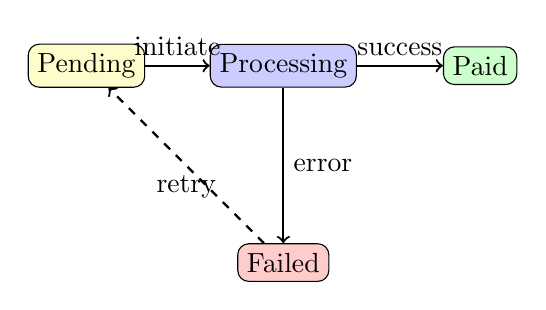
\begin{tikzpicture}[node distance=2.5cm, auto]
    \node[draw, rounded corners, fill=yellow!20] (pending) {Pending};
    \node[draw, rounded corners, fill=blue!20, right of=pending] (processing) {Processing};
    \node[draw, rounded corners, fill=green!20, right of=processing] (paid) {Paid};
    \node[draw, rounded corners, fill=red!20, below of=processing] (failed) {Failed};
    
    \draw[->, thick] (pending) -- node[above] {initiate} (processing);
    \draw[->, thick] (processing) -- node[above] {success} (paid);
    \draw[->, thick] (processing) -- node[right] {error} (failed);
    \draw[->, thick, dashed] (failed) -- node[below] {retry} (pending);
\end{tikzpicture}
\end{center}

\textbf{Rule:} Only orders in ``Pending'' state can be processed. Orders in ``Processing'' or ``Paid'' states reject new payment attempts.

% IMAGE 4: bKash Payment
\begin{figure}[H]
    \centering
    \includegraphics[width=0.9\textwidth]{results/bkash_payment.png}
    \caption{bKash Mobile Banking Payment Flow}
    \label{fig:bkash}
\end{figure}

% ============================================
% 5. HANDLING SLOW EXTERNAL SERVICES (2.0 Marks - Resilience)
% ============================================
\section{Handling Slow External Services}

External payment gateways (bKash, Nagad, bank APIs) may experience delays. Our resilience strategies include:

\subsection{Timeout Configuration}

\begin{itemize}
    \item Connection timeout: 5 seconds
    \item Response timeout: 30 seconds
    \item If timeout occurs, return ``pending'' status to user
\end{itemize}

\subsection{Retry with Exponential Backoff}

\begin{verbatim}
async function retryPayment(fn, maxRetries = 3) {
    for (let attempt = 1; attempt <= maxRetries; attempt++) {
        try {
            return await fn();
        } catch (error) {
            const delay = Math.pow(2, attempt) * 1000; // 2s, 4s, 8s
            await sleep(delay);
        }
    }
    throw new Error('Payment gateway unavailable');
}
\end{verbatim}

\subsection{Background Processing (Asynchronous)}

\begin{enumerate}
    \item User submits payment $\rightarrow$ System immediately returns ``Processing''
    \item Payment is added to a message queue (e.g., Redis Queue)
    \item Background worker processes payment
    \item User is notified via push notification/SMS when complete
\end{enumerate}

\subsection{Circuit Breaker Pattern}

If a payment gateway fails repeatedly, the circuit ``opens'' and subsequent requests immediately fail-fast:

\begin{center}
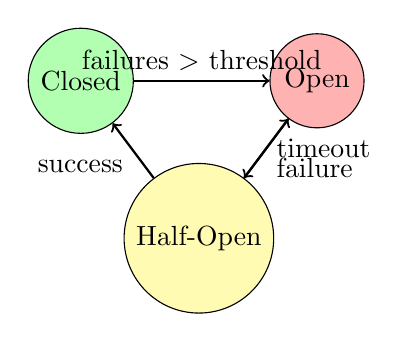
\begin{tikzpicture}[node distance=3cm, auto]
    \node[draw, circle, fill=green!30] (closed) {Closed};
    \node[draw, circle, fill=red!30, right of=closed] (open) {Open};
    \node[draw, circle, fill=yellow!30, below of=open, yshift=1cm, xshift=-1.5cm] (half) {Half-Open};
    
    \draw[->, thick] (closed) -- node[above] {failures $>$ threshold} (open);
    \draw[->, thick] (open) -- node[right] {timeout} (half);
    \draw[->, thick] (half) -- node[below left] {success} (closed);
    \draw[->, thick] (half) -- node[below right] {failure} (open);
\end{tikzpicture}
\end{center}

% ============================================
% 6. BALANCING STAKEHOLDER NEEDS
% ============================================
\section{Balancing Stakeholder Needs}

\textbf{Challenge:} Customers want instant payment confirmation, while auditors require comprehensive transaction logs. These seem conflicting because logging can slow down response times.

\textbf{Solution:} We implement \textbf{asynchronous logging with synchronous confirmation}:

\begin{enumerate}
    \item Payment processing completes and customer receives immediate confirmation (synchronous, fast)
    \item Detailed audit logs are written asynchronously to a separate logging service in the background
    \item Audit service maintains complete immutable logs without affecting payment response time
\end{enumerate}

This approach satisfies both stakeholders: customers experience sub-second confirmations, while auditors have access to comprehensive transaction histories stored in a separate audit database with 7-year retention.

% IMAGE 5: Payment Success
\begin{figure}[H]
    \centering
    \includegraphics[width=0.9\textwidth]{results/payment_success.png}
    \caption{Payment Successful Confirmation Screen}
    \label{fig:success}
\end{figure}

% ============================================
% 7. SYSTEM ARCHITECTURE DIAGRAM (2.0 Marks)
% ============================================
\section{System Architecture Diagram}

\subsection{Use Case Diagram}

\begin{center}
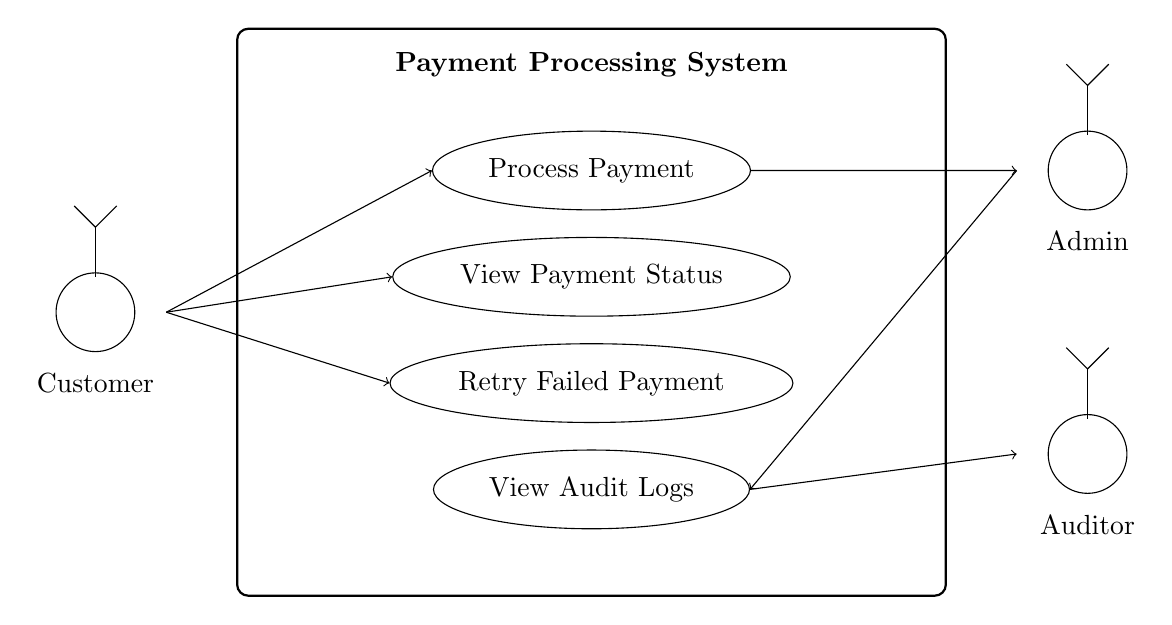
\begin{tikzpicture}[scale=0.9]
    % System boundary
    \draw[thick, rounded corners] (0,0) rectangle (10,8);
    \node at (5,7.5) {\textbf{Payment Processing System}};
    
    % Actors
    \node[draw, circle, minimum size=1cm] (customer) at (-2, 4) {};
    \node at (-2, 3) {Customer};
    \draw (-2, 4.5) -- (-2, 5.2);
    \draw (-2.3, 5.5) -- (-2, 5.2) -- (-1.7, 5.5);
    
    \node[draw, circle, minimum size=1cm] (admin) at (12, 6) {};
    \node at (12, 5) {Admin};
    \draw (12, 6.5) -- (12, 7.2);
    \draw (11.7, 7.5) -- (12, 7.2) -- (12.3, 7.5);
    
    \node[draw, circle, minimum size=1cm] (auditor) at (12, 2) {};
    \node at (12, 1) {Auditor};
    \draw (12, 2.5) -- (12, 3.2);
    \draw (11.7, 3.5) -- (12, 3.2) -- (12.3, 3.5);
    
    % Use cases
    \node[draw, ellipse, minimum width=3cm, minimum height=1cm] (uc1) at (5, 6) {Process Payment};
    \node[draw, ellipse, minimum width=3cm, minimum height=1cm] (uc2) at (5, 4.5) {View Payment Status};
    \node[draw, ellipse, minimum width=3cm, minimum height=1cm] (uc3) at (5, 3) {Retry Failed Payment};
    \node[draw, ellipse, minimum width=3cm, minimum height=1cm] (uc4) at (5, 1.5) {View Audit Logs};
    
    % Connections
    \draw[->] (-1, 4) -- (uc1.west);
    \draw[->] (-1, 4) -- (uc2.west);
    \draw[->] (-1, 4) -- (uc3.west);
    \draw[->] (uc1.east) -- (11, 6);
    \draw[->] (uc4.east) -- (11, 2);
    \draw[->] (11, 6) -- (uc4.east);
\end{tikzpicture}
\end{center}

\subsection{Component Diagram}

\begin{center}
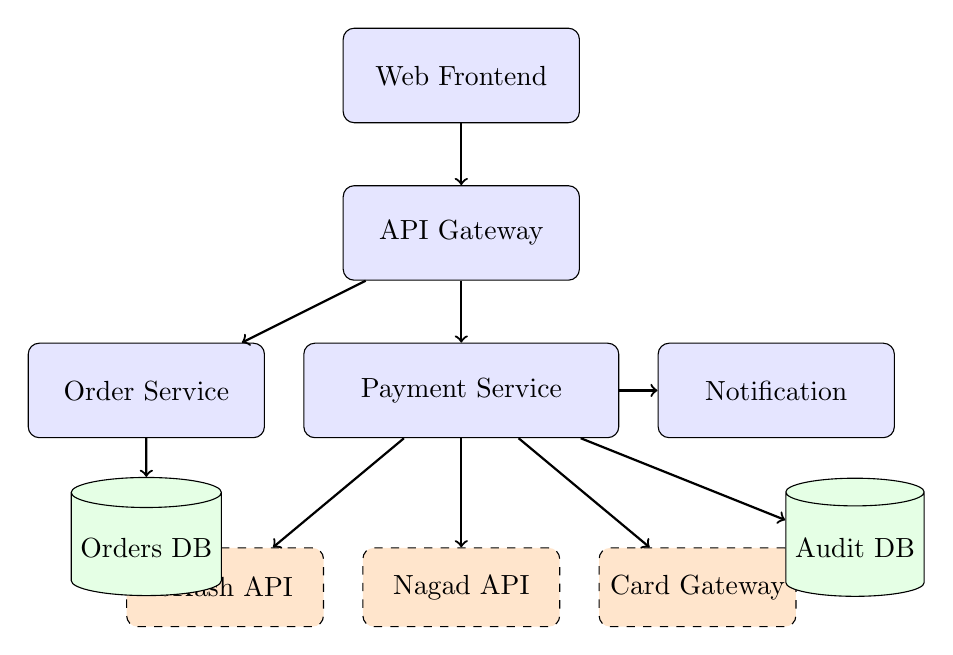
\begin{tikzpicture}[
    component/.style={draw, rectangle, rounded corners, minimum width=3cm, minimum height=1.2cm, fill=blue!10},
    database/.style={draw, cylinder, shape border rotate=90, aspect=0.2, minimum height=1.5cm, minimum width=1.5cm, fill=green!10},
    external/.style={draw, rectangle, rounded corners, minimum width=2.5cm, minimum height=1cm, fill=orange!20, dashed}
]
    % Frontend
    \node[component] (frontend) at (0, 4) {Web Frontend};
    
    % API Gateway
    \node[component] (api) at (0, 2) {API Gateway};
    
    % Payment Service
    \node[component, minimum width=4cm] (payment) at (0, 0) {Payment Service};
    
    % Order Service
    \node[component] (order) at (-4, 0) {Order Service};
    
    % Notification Service
    \node[component] (notif) at (4, 0) {Notification};
    
    % External Gateways
    \node[external] (bkash) at (-3, -2.5) {bKash API};
    \node[external] (nagad) at (0, -2.5) {Nagad API};
    \node[external] (card) at (3, -2.5) {Card Gateway};
    
    % Databases
    \node[database] (ordersdb) at (-4, -2) {Orders DB};
    \node[database] (auditdb) at (5, -2) {Audit DB};
    
    % Arrows
    \draw[->, thick] (frontend) -- (api);
    \draw[->, thick] (api) -- (payment);
    \draw[->, thick] (api) -- (order);
    \draw[->, thick] (payment) -- (notif);
    \draw[->, thick] (payment) -- (bkash);
    \draw[->, thick] (payment) -- (nagad);
    \draw[->, thick] (payment) -- (card);
    \draw[->, thick] (order) -- (ordersdb);
    \draw[->, thick] (payment) -- (auditdb);
    
\end{tikzpicture}
\end{center}

% IMAGE 6: Admin Dashboard
\begin{figure}[H]
    \centering
    \includegraphics[width=0.9\textwidth]{results/admin_orders.png}
    \caption{Admin Dashboard Showing Payment Tracking and Audit Information}
    \label{fig:admin}
\end{figure}

% ============================================
% 8. CONCLUSION
% ============================================
\section{Conclusion}

This document presents a comprehensive design for the payment processing module of the Bongoportus e-commerce platform. Key design decisions include:

\begin{itemize}
    \item \textbf{Agile methodology} for iterative development with stakeholder feedback
    \item \textbf{Idempotency keys} and \textbf{database locking} to prevent duplicate payments
    \item \textbf{Retry mechanisms} and \textbf{circuit breakers} for resilience against slow external services
    \item \textbf{Asynchronous logging} to balance fast customer experience with comprehensive auditing
\end{itemize}

The system is designed to handle high concurrent loads during flash sales while maintaining security, reliability, and compliance with financial regulations.

% ============================================
% GRADING RUBRIC COMPLIANCE
% ============================================
\section*{Rubric Compliance Summary}

\begin{table}[H]
\centering
\begin{tabular}{|l|c|l|}
\hline
\textbf{Criteria} & \textbf{Marks} & \textbf{Section Reference} \\
\hline
Process Model & 2.0 & Section 2: Agile with stakeholder/reliability justification \\
\hline
Requirements & 2.0 & Section 3: 4 FR + 4 NFR as specified \\
\hline
Payment Logic & 2.0 & Section 4: Idempotency + Transaction rules \\
\hline
Resilience & 2.0 & Section 5: Retry, timeout, circuit breaker \\
\hline
Diagramming & 2.0 & Section 7: Use Case + Component diagrams \\
\hline
\end{tabular}
\caption{Grading Rubric Compliance}
\end{table}

% ============================================
% REFERENCES
% ============================================
\section*{References}

\begin{enumerate}
    \item Sommerville, I. (2016). \textit{Software Engineering} (10th ed.). Pearson.
    \item Fowler, M. (2018). \textit{Patterns of Enterprise Application Architecture}. Addison-Wesley.
    \item bKash Developer Documentation. https://developer.bkash.com
    \item PCI Security Standards Council. \textit{PCI DSS Requirements}. https://www.pcisecuritystandards.org
\end{enumerate}

\end{document}
